\chapter{Supplementary for Chapter 2} \label{app-tephra}


\section{Q-Q plots for MAE and MAPE}\label{supp-a}
    
    % Additional plots for cost function selection
    \begin{figure}[htbp]
    \centering
    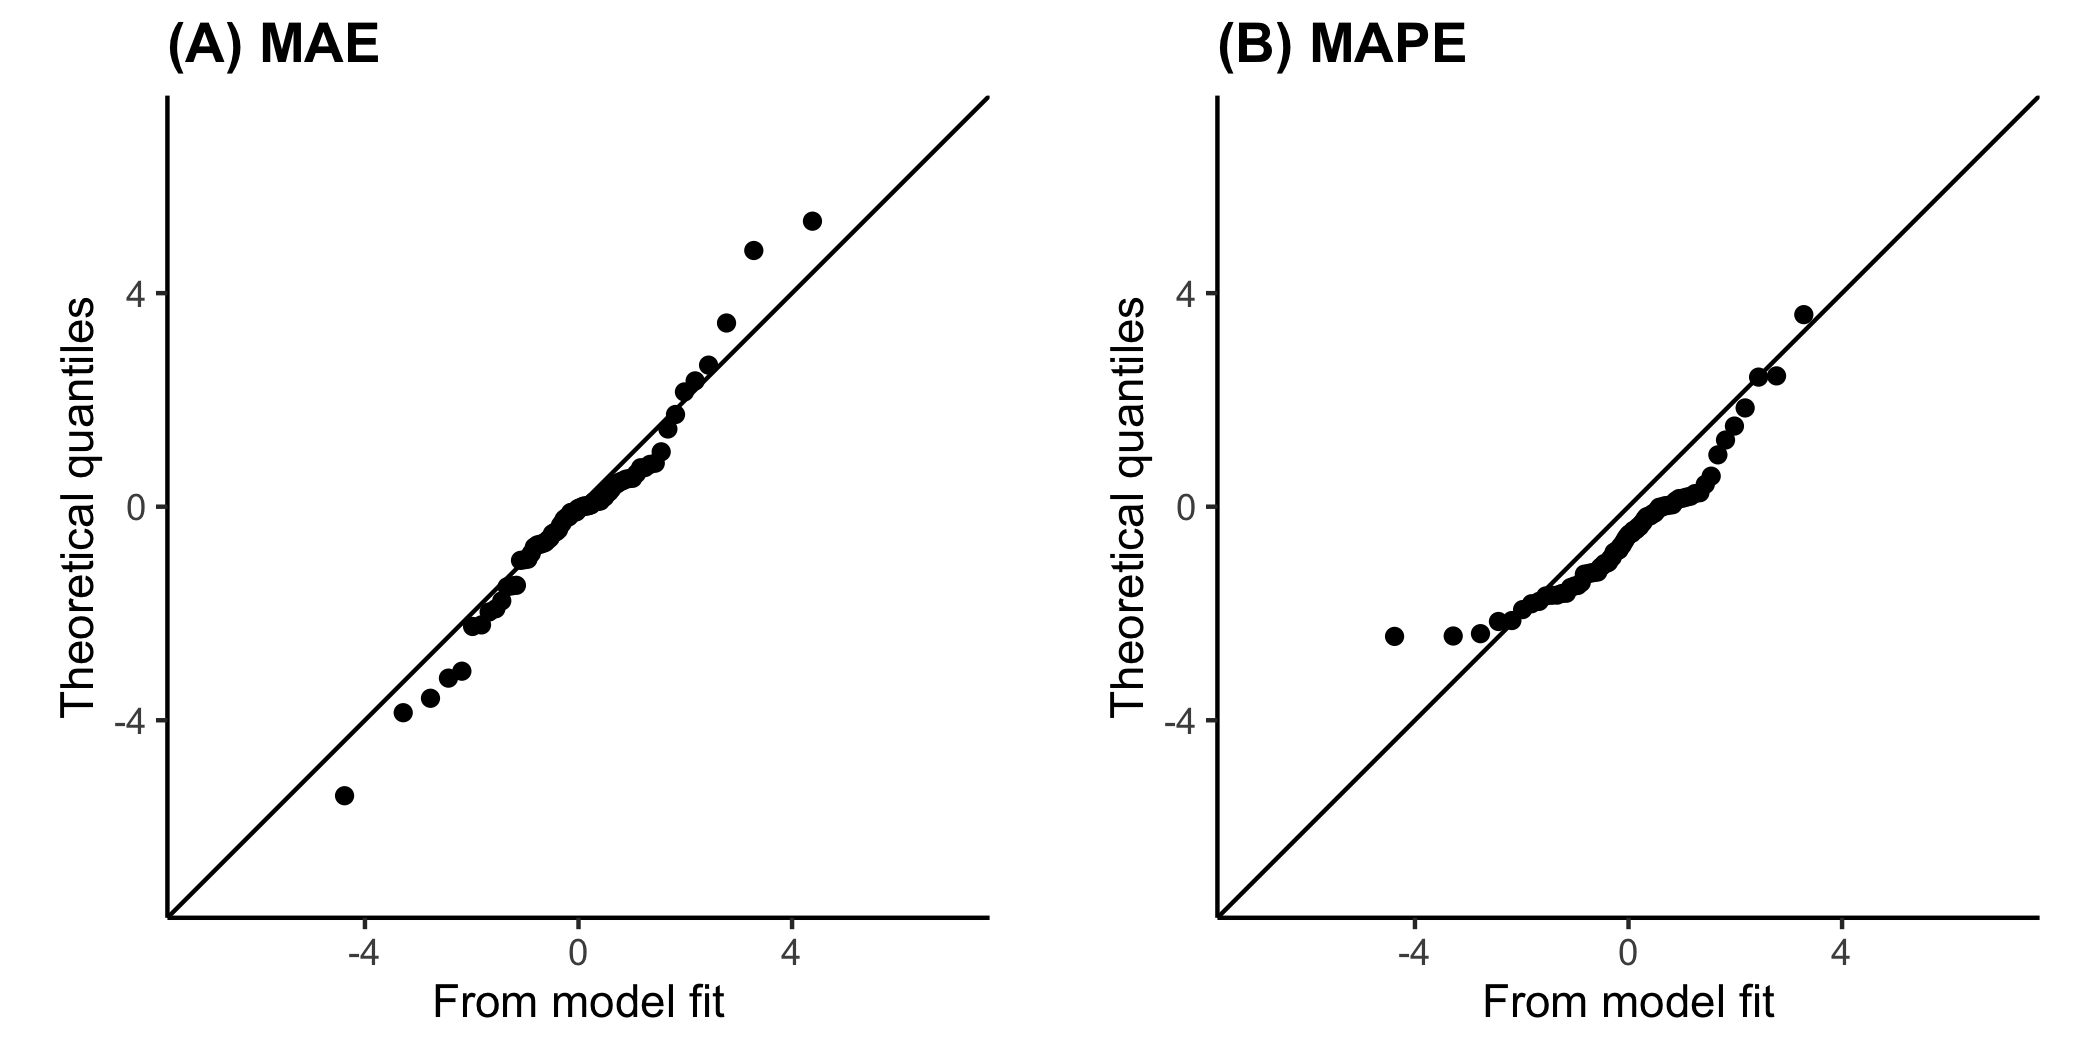
\includegraphics[width=0.9\linewidth]{Figures/fig10_qq-plots-others.png}
    \caption{Quantile-quantile (Q-Q) plots illustrating goodness-of-fit for the different models fitted using different cost functions: mean absolute error (MAE) and mean absolute percentage error (MAPE). The fit is evaluated by how well the empirical quantiles from the transformed model residuals line up with the theoretical quantiles from the assumed distributions along the diagonal line.}
    \end{figure}

\section{MSLE vs. MAPE}\label{supp-b}
    
    A widely-used order-dependent cost function is the mean absolute percentage error (MAPE), which is obtained by aggregating the relative errors using the mean and then converting to a percentage: 
    
    \begin{equation}
    \frac{100}{n} \sum_{i=1}^{n} \left | \frac{\varepsilon_{i}}{x_{i}}  \right |
    \end{equation}
    
    MAPE is used in different areas of research such as atmospheric science and space science (e.g., \cite{grillakis2013multisegment, zheng2015linear, zhelavskaya2016automated}). Despite being easy to interpret due to its usage of the percentage, MAPE has been proven to have problems when used in model calibration:
    
    \begin{enumerate}
    
        \item MAPE is asymmetric with respect to overestimation and underestimation (Hyndman \& Koehler, 2006; Makridakis, 1993; Tofallis, 2015).
        
        \item MAPE is constrained to be positive, so its distribution is generally positively skewed (Hyndman \& Koehler, 2006; Swanson et al., 2000).
        
        \item MAPE becomes undefined when the true value is zero (Hyndman \& Koehler, 2006). 
        
        \item MAPE is not resistant to outliers (Swanson et al., 2000; Tofallis, 2015).
        
    \end{enumerate}
    
    To elaborate on the first point, a prediction of 100 where the observed value is 50 gives a different magnitude of error (100\%) than a prediction of 50 where the observed value is 100 (50\%). Underprediction is therefore less heavily penalized than overprediction, even if the order of the error is the same. The third point also means that MAPE is not an appropriate metric where the quantity being predicted is likely to be zero (e.g., \cite{tofallis2015better}).%%%%rephrase??
    

\section{Simple kriging interpolation}\label{supp-c}

The procedure for simple kriging interpolation is as follows:

\begin{enumerate}

    \item For each pair of residuals at the sampled sites, calculate the variogram value $\gamma$ as half of the mean-squared difference between their values. 
    
    \item Define a model of spatial variation (i.e. variogram model) that best relates the variogram values from Step 1, and the corresponding separation distances ($h$) for each pair of locations. The variogram model's parameters may be user-defined or estimated using a maximum likelihood estimation approach. In defining the variogram model, we adopt the Mat\'ern function, and use the geostats and geoR packages in R programming environment for fitting \citep{diggle2007, georpackage2001, geostatsRpkg, rpackage2006}. 
    
    \item Estimate the elements of the covariance matrix, $\Sigma$, which describes the spatial relationships among the values at the observed sites and the prediction location. The covariance matrix has a size of $N \times N$, and its $i-j$th element is defined as 
    \begin{equation}
    c(s_{i}, s_{j}) = \sigma^{2}\gamma(h) + \tau^2,
    \end{equation} \label{eq:cov}
    where $\sigma^2$ is the amount of spatially correlated variation, $\gamma(h)$ is the variogram model from Step 2, $\tau^2$ is the variogram value at zero separation distance, and $h$ is the distance between the two observation sites $s_{i}$ and $s_{j}$. The parameters $\sigma^2$ and $\tau^2$ are derived from the variogram model. The variable $\tau^2$ is more commonly known as the \textit{nugget} in the geostatistics literature, and it represents the variability in the interpolated at very short separation distances. 
    
    \item Calculate kriging weights $\lambda_{i}$ as:
    \begin{equation}
    \begin{pmatrix}
    \lambda_{1}\\ 
    \vdots \\ 
    \lambda_{N}
    \end{pmatrix}   = 
    \begin{pmatrix}
    c(s_{1}, s_{1}) &  \cdots & c(s_{1}, s_{N})  \\ 
    \vdots & \ddots  & \vdots\\ 
    c(s_{N}, s_{1}) & \cdots  & c(s_{N}, s_{N})  
    \end{pmatrix}^{-1}
    \begin{pmatrix}
    c(s_{1}, s_{0})\\ 
    \vdots \\ 
    c(s_{N}, s_{0})
    \end{pmatrix} 
    \end{equation} \label{eq:cov}    
    
    \item Calculate the residual for all sites in the study area. The residual at any prediction location $s_{o}$ can be written as:
    \begin{equation}
    \hat{Z}(s_{o}) = \sum_{i=1}^{N} \lambda_{i} Z(s_{i}) 
    \end{equation} \label{eq:simpkrig-app}

    where $Z(s_{i})$ is the residual at an observed location $s_{i}$ calculated using the equations for $Z_{i} in Table \ref{tab:costf}$, $\lambda_{i}$ is the weight applied to the value at the observed location, and $N$ is the number of observed sites. 
    
 
    
    \item The associated kriging error can be calculated as:
    
    \begin{equation}
    Var( \hat{Z}(s_{o})-  Z(s_{o}) )=
    c(s_{0}, s_{0}) - 
    \begin{pmatrix}
    c(s_{1}, s_{0})\\ 
    \vdots \\ 
    c(s_{N}, s_{0})
    \end{pmatrix}^{'} 
    \begin{pmatrix}
    c(s_{1}, s_{1}) &  \cdots & c(s_{1}, s_{N})  \\ 
    \vdots & \ddots  & \vdots\\ 
    c(s_{N}, s_{1}) & \cdots  & c(s_{N}, s_{N})  
    \end{pmatrix}^{-1}
    \begin{pmatrix}
    c(s_{1}, s_{0})\\ 
    \vdots \\ 
    c(s_{N}, s_{0})
    \end{pmatrix} 
    \end{equation} 
 
    
\end{enumerate}


\section{Back transformation}\label{supp-c-back}

If MSE was used as the cost function in the inversion, the final prediction map can be written as $\widehat{Y} = \mu + \hat{\epsilon}$ where $\mu$ denotes the forward model prediction. The associated spatial prediction uncertainty $Var[\widehat{Y}(\mathbf{x})]$ is equivalent to $Var\left[\epsilon(\mathbf{x})|\epsilon(\mathbf{x}_{1}), \dots, \epsilon(\mathbf{x}_{N})\right]$.

For the other cost functions related to Gaussian distributions, namely the chi-square error and MSLE, we can transform the residuals as outlined in Table \ref{tab:GOF_loss} before applying simple kriging. We would then need to back-transform the predicted residuals and their prediction errors to obtain the final prediction maps. 
\\
For chi-square loss:
\begin{gather}
\widehat{Y} = \mu + \sqrt{\mu}\hat{\epsilon} \text{ and }
Var[\widehat{Y}] = \mu Var[\hat{\epsilon}]. \label{eqn:chisquarebt}
\end{gather}

For MSLE:
\begin{align}
\widehat{Y} &= \exp\left(\frac{\log_{10}\left(\mu + 1\right) - \hat{\epsilon}}{\log_{10}e} + \frac{\Var\left[\epsilon(\mathbf{x})|\epsilon(\mathbf{x}_{1}), 
    \dots, \epsilon(\mathbf{x}_{N})\right]}{2(\log_{10}e)^2}\right) - 1 \label{eqn:mslbt1} \\
\text{and } Var[\widehat{Y}] &= \left[\exp\left(\frac{\Var\left[\epsilon(\mathbf{x})|\epsilon(\mathbf{x}_{1}), 
    \dots, \epsilon(\mathbf{x}_{N})\right]}{(\log_{10}e)^2}\right) - 1\right]\exp\left(2\frac{\log_{10}(\mu + 1) - \hat{\epsilon}}{\log_{10}e} + \frac{\Var\left[\epsilon(\mathbf{x})|\epsilon(\mathbf{x}_{1}), 
    \dots, \epsilon(\mathbf{x}_{N})\right]}{(\log_{10}e)^2}\right) \label{eqn:mslbt2}
\end{align}

A derivation of the prediction formulae for MSLE is given in Section \ref{supp-c-msle}.

%%%%%%%%%%%%%%%%%%%%%%%%%%%%%%%%%%%%%%%%%%%%%
\section{Derivation of the MSLE prediction formulae} \label{supp-c-msle}
%%%%%%%%%%%%%%%%%%%%%%%%%%%%%%%%%%%%%%%%%%%%%

When we use mean squared logarithmic error (MSLE) as a loss function to calibrate our forward model, we are implicitly assuming a Gaussian distribution on its transformed residual $Z_{i} = \log_{10}\left(\frac{Predicted + 1}{Actual + 1}\right)$ where $Predicted = \mu$ is the forward model prediction and $Actual$ is the observed tephra load (see Table \ref{tab:costf} in the Main Paper). Hence, to model spatial deviations from the forward model, we conduct simple kriging or the method in \cite{worden2018} on the transformed residuals. 
\\
Let $\hat{\epsilon} = \mathbb{E}\left[\epsilon(\mathbf{x})|\epsilon(\mathbf{x}_{1}), 
    \dots, \epsilon(\mathbf{x}_{N})\right]$ denote the kriging prediction and $\Var\left[\epsilon(\mathbf{x})|\epsilon(\mathbf{x}_{1}), 
    \dots, \epsilon(\mathbf{x}_{N})\right]$ the prediction variance. Then:
\begin{gather}
    \log_{10}\left(Actual + 1\right) \sim N(\log_{10}\left(Predicted + 1\right) - \hat{\epsilon}, \Var\left[\epsilon(\mathbf{x})|\epsilon(\mathbf{x}_{1}), 
    \dots, \epsilon(\mathbf{x}_{N})\right]),
\end{gather}
since $\log_{10}\left(Actual + 1\right) = \log_{10}\left(Predicted + 1\right) - \log_{10}\left(\frac{Predicted + 1}{Actual + 1}\right)$. 
\\
Change bases from $10$ to $e$, we have:
\begin{gather}
    \log_{e}\left(Actual + 1\right) = \frac{\log_{10}\left(Actual + 1\right)}{\log_{10}\left(e\right)} \sim N\left(\frac{\log_{10}\left(Predicted + 1\right) - \hat{\epsilon}}{\log_{10}\left(e\right)}, \frac{\Var\left[\epsilon(\mathbf{x})|\epsilon(\mathbf{x}_{1}), 
    \dots, \epsilon(\mathbf{x}_{N})\right]}{\left(\log_{10}\left(e\right)\right)^2}\right),
\end{gather}
This means that $Actual + 1 \sim logNormal\left(\frac{\log_{10}\left(Predicted + 1\right) - \hat{\epsilon}}{\log_{10}\left(e\right)}, \frac{\Var\left[\epsilon(\mathbf{x})|\epsilon(\mathbf{x}_{1}), 
    \dots, \epsilon(\mathbf{x}_{N})\right]}{\left(\log_{10}\left(e\right)\right)^2}\right)$. 
Using the formulae for the mean and the variance of a logNormal random variable, and writing $Predicted$ as $\mu$, the estimated tephra load and its prediction variance are:
\begin{align}
\widehat{Y} &= \exp\left(\frac{\log_{10}\left(\mu + 1\right) - \hat{\epsilon}}{\log_{10}e} + \frac{\Var\left[\epsilon(\mathbf{x})|\epsilon(\mathbf{x}_{1}), 
    \dots, \epsilon(\mathbf{x}_{N})\right]}{2(\log_{10}e)^2}\right) - 1 \\
\text{and } \Var[\widehat{Y}] &= \left[\exp\left(\frac{\Var\left[\epsilon(\mathbf{x})|\epsilon(\mathbf{x}_{1}), 
    \dots, \epsilon(\mathbf{x}_{N})\right]}{(\log_{10}e)^2}\right) - 1\right]\exp\left(2\frac{\log_{10}(\mu + 1) - \hat{\epsilon}}{\log_{10}e} + \frac{\Var\left[\epsilon(\mathbf{x})|\epsilon(\mathbf{x}_{1}), 
    \dots, \epsilon(\mathbf{x}_{N})\right]}{(\log_{10}e)^2}\right).
\end{align}


\section{LOOCV procedure} \label{supp-loocv}


    LOOCV computes the test performance for all reference data points. The following steps are conducted for both the simple kriging in Section \ref{subsection-kriging-interp}, and its extension in Section \ref{subsection-kriging-worden} which accounts for varying data uncertainty: 
  
        \begin{enumerate}
  
        \item We make use of the transformed residuals at the observation sites calculated in Section \ref{subsection-kriging-interp} Step 2a. For brevity in the steps that follow, we refer to the transformed residual at an observation site as \textit{observation point}.
    
        \item We set aside one observation point as a test point, while the other observation points form the training set. Note that we only use observation points from the reference dataset (i.e. Dataset 1) as test set. The idea is to evaluate the performance of the interpolation approach on the most reliable data.
  
        \item Using only the training points, kriging interpolation is conducted for the test point.
    
        \item This interpolated value of transformed residual is combined to the optimised model estimate for the test location following Section \ref{subsection-kriging-interp}'s Steps 3a and 3b. The result is an updated value of tephra load at test site. 
    
        \item The above steps are repeated until all points from Dataset 1 are evaluated as a test point. For all iterations, the interpolated load estimates are compared against the observed tephra load values based on a performance metric (e.g. root mean square error, chi-square, and mean square log error). The result is the LOOCV error associated with the kriging interpolation approach used in Step 3.

        \end{enumerate}
  
  
\section{Checks for isotropy and residual form} \label{supp-isotrop}

    We investigate the strength of the spatial correlation when the residuals are transformed in different forms, with the aim of finding which residual form is best for the kriging methods. We hypothesize that the log-residual is more suitable for use in kriging, since in Section \ref{subsection-res-costf}, we identified that MSLE is the most suitable cost function for the case study. 

    In Figure \ref{fig:vars_three}, we show the empirical and fitted variograms for the different forms of residuals. Annotated in the figures are the variograms' \textit{range}, which vary across the variogram models shown. For instance, the range up to which log residuals can be interpolated (around 22km) was around three times larger than for the actual residuals (around 7km). This indicates that the log residuals are more appropriate to interpolate the residuals. Because of this evidence, we proceed with using log residuals for the spatial interpolation of the model deviations. 

    \begin{figure*}[htbp!]
    \centering
    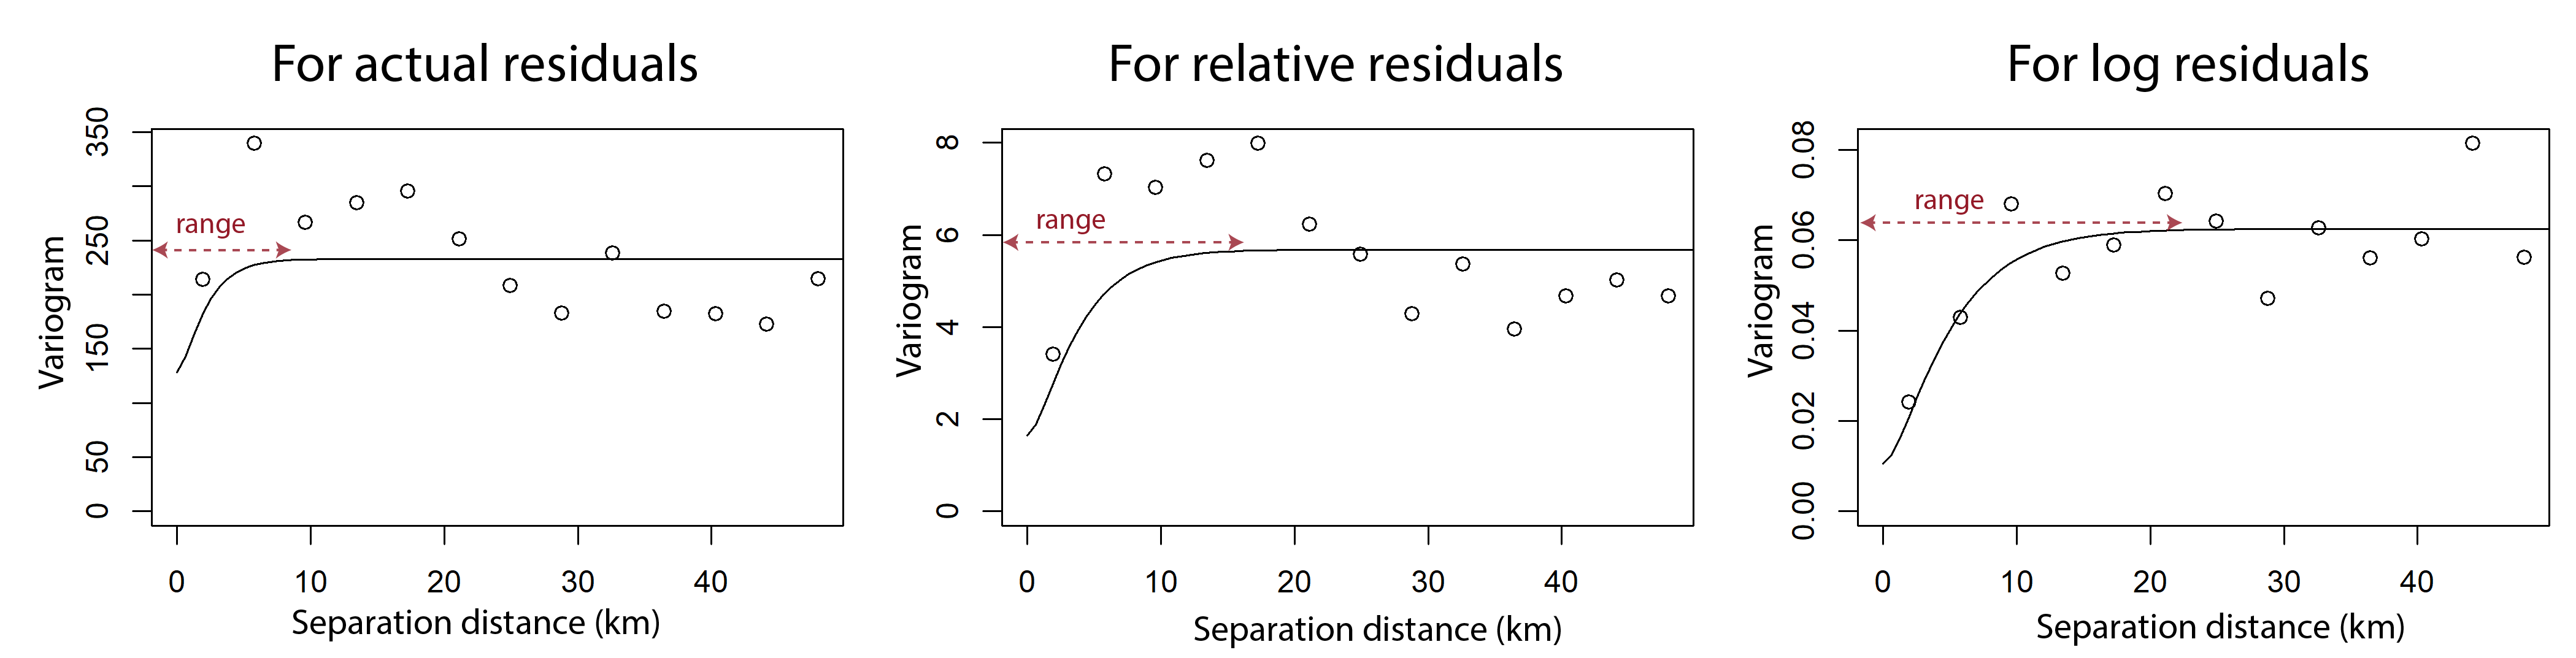
\includegraphics[width=\linewidth]{Figures/fig11_variograms-types.png}
    \caption{Empirical and fitted Mat\'ern variogram for actual and log residuals. Note that the widely different range of semivariance values in the y-axis is due to the scale of which the residuals are transformed. The range of the variograms (indicated with a dotted line) indicate the lag distances where data is spatially correlated. Beyond the range, interpolation does not occur.}
    \label{fig:vars_three}
    \end{figure*}
    
    We also confirmed the validity of assuming an isotropic field when modelling the spatial correlation, for which we use directional variograms. This step serves as a statistical check of the assumptions made in the kriging methodology since exterior factors (i.e. related to the physics of tephra deposition) may affect the spatial structure of the dataset and the model deviations. To generate the directional variograms, the variance for pairs of data were calculated for specific directions within a certain tolerance. Since the correlation structure appears similar for all the directional variograms in Figure \ref{fig:vars_direct}, there's no evidence of anisotropy. Hence, the assumption of an isotropic field is acceptable.
    
    \begin{figure*}[htbp!]
    \centering
    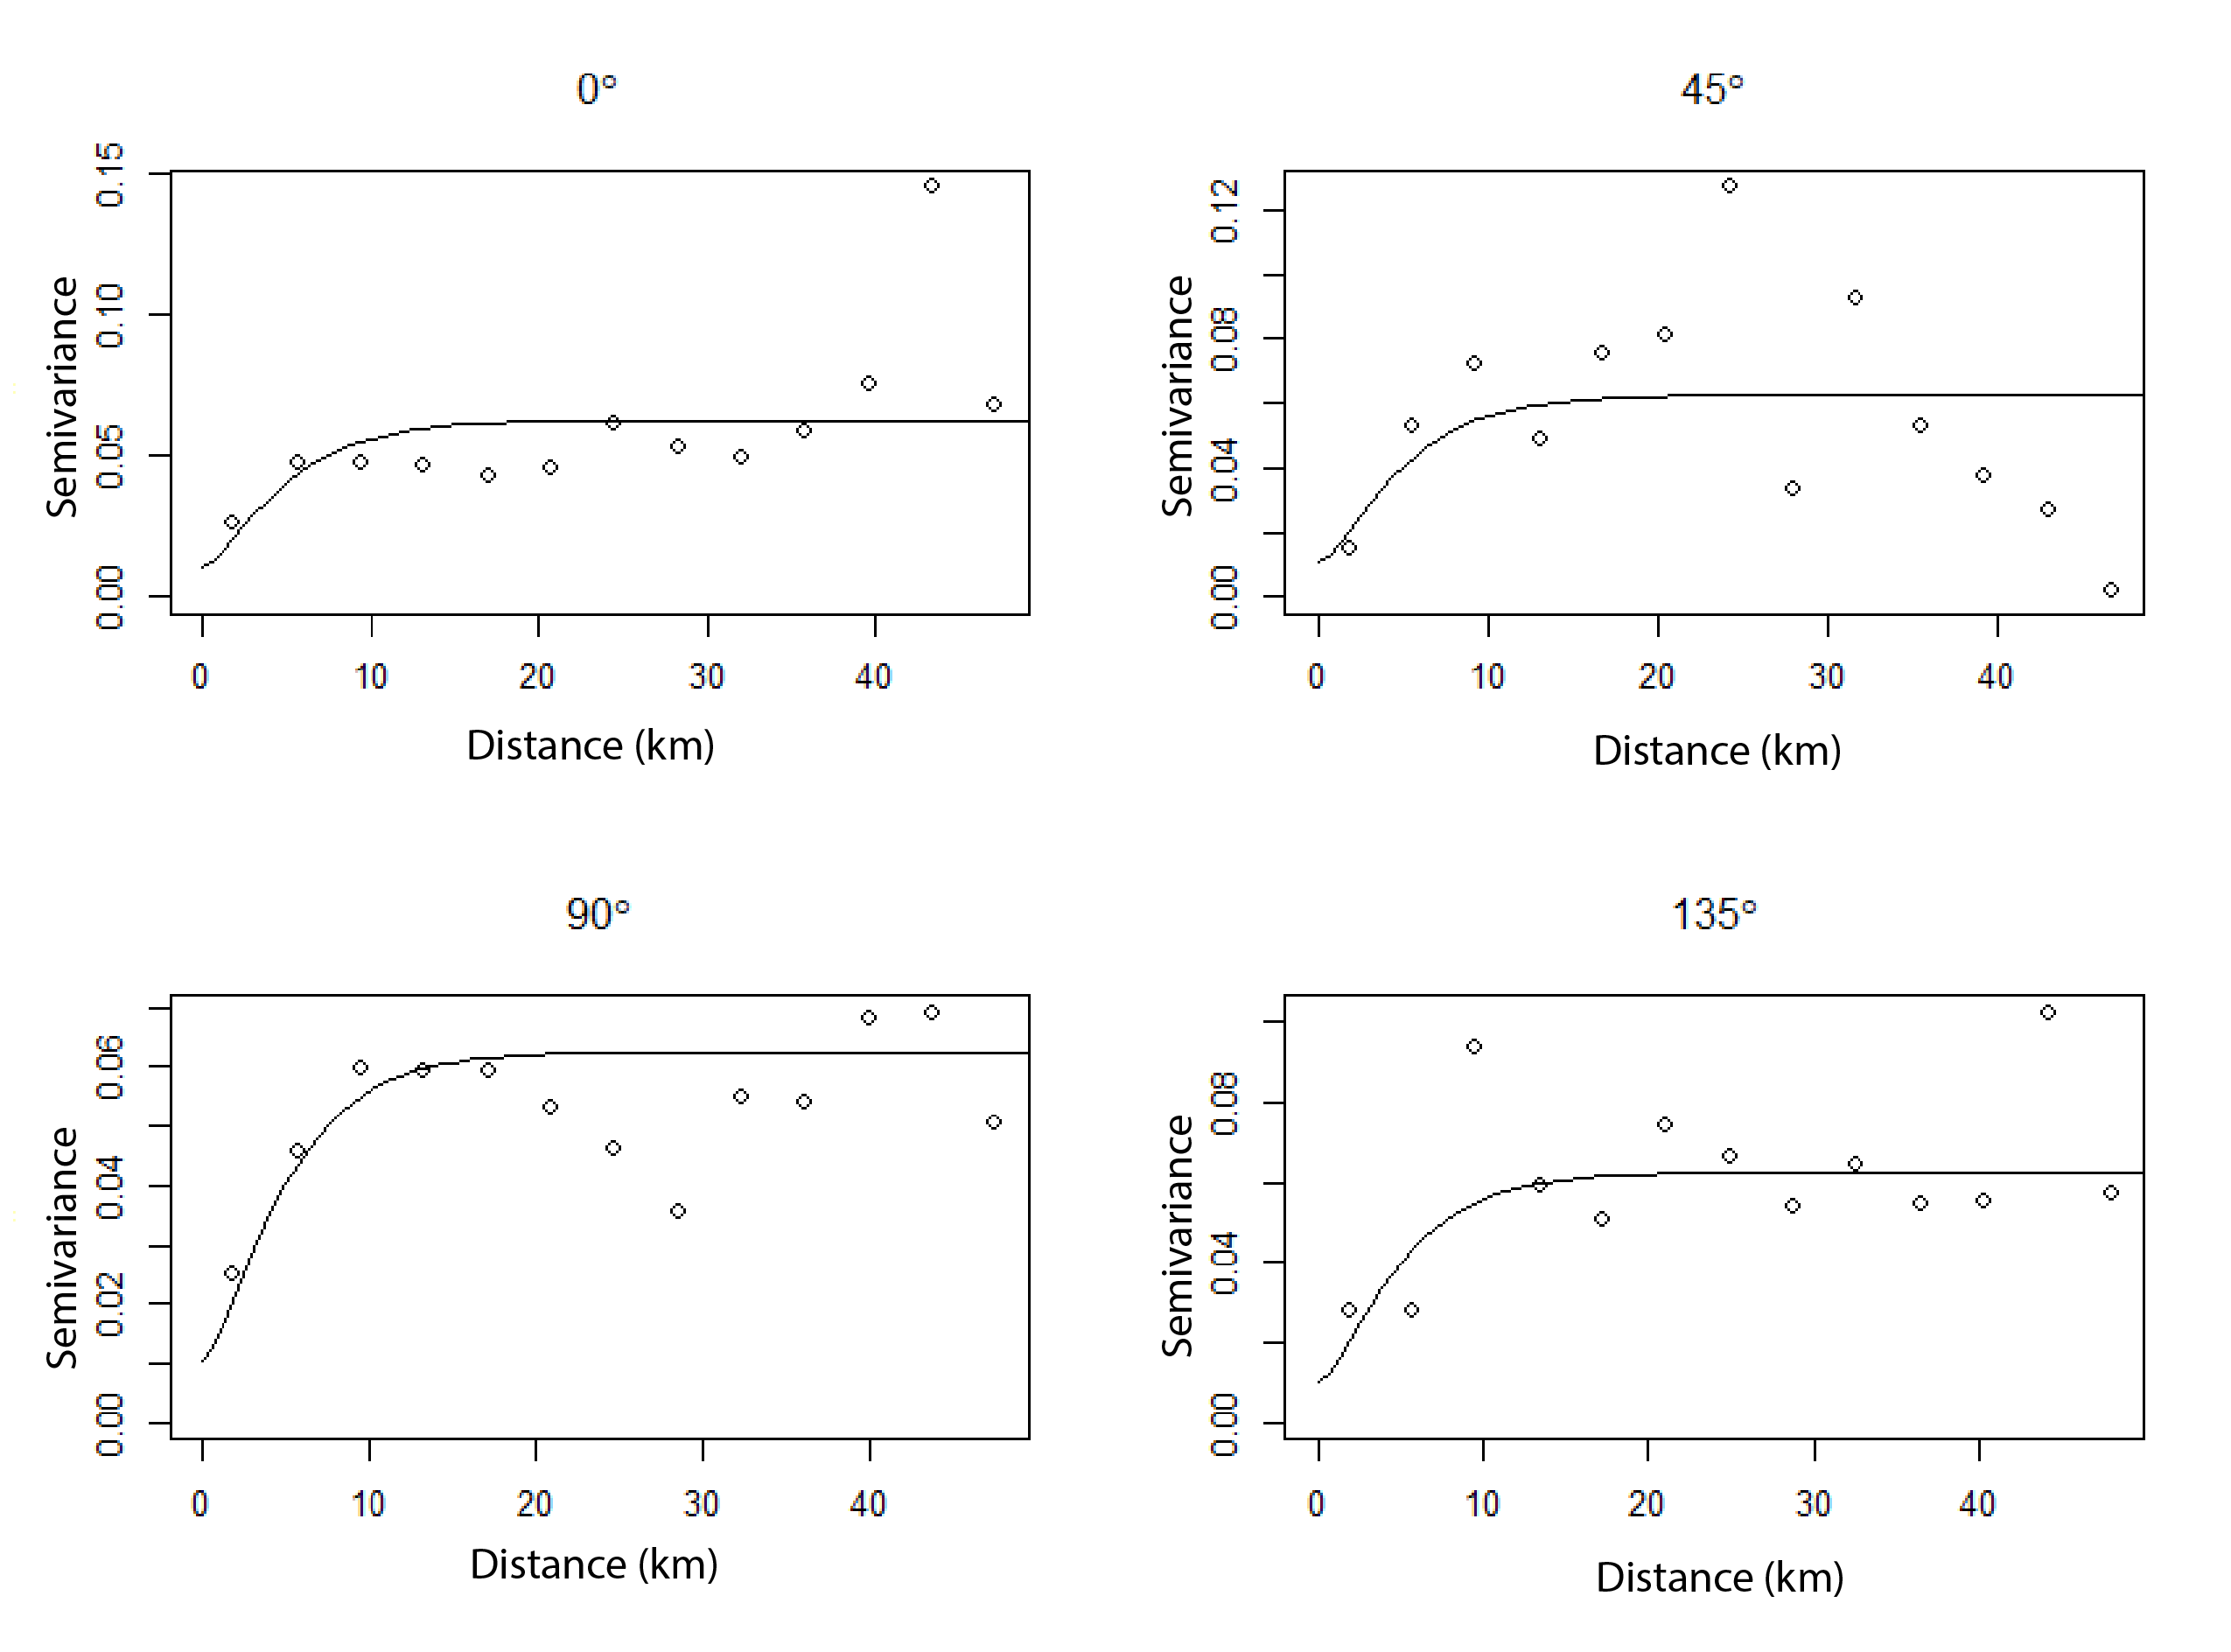
\includegraphics[width=\linewidth]{Figures/fig12_variograms-directions.png}
    \caption{The fitted omnidirectional Mat\'ern model (shown in solid line) and empirical directional variograms (points) for the directions N0E, N45E, N90E, and N135E. An angular tolerance of 22.5 is set for generating the directional variograms.}
    \label{fig:vars_direct}
    \end{figure*}
  
%----------------

\section{Leave-one-out cross-validation errors from fusion with different variogram models}\label{supp-e}

Table \ref{tab:supp-allvarmods} shows the leave-one-out cross-validation (LOOCV) errors after weighted and unweighted fusion. For all cost functions and variogram models considered except the case of the Gaussian model for the chi-square cost function, the errors are lower for weighted fusion as compared to those from the unweighted fusion. In addition, the LOOCV errors are lower than the pre-kriging training error, indicating that there was no overfitting due to kriging. 


\afterpage{%
    \clearpage% Flush earlier floats (otherwise order might not be correct)
    \begin{landscape}% Landscape page
%%%%%%%%%%%%%%%%%%%%%
    \begin{table}[]
    \centering
    \caption{Measures of performance of the unweighted and weighted kriging-based fusion methods in terms of LOOCV errors for different variogram models. The errors were calculated using three different metrics with formulas indicated in the table: root mean squared errors, chi-square errors and mean square log error. The training errors before applying the fusion methods are consistently higher than the LOOCV errors, which indicates no overfitting in the kriging method.}
    \label{tab:supp-allvarmods}
    \begin{tabular}{@{}lllccc@{}}
    \toprule
    \multirow{2}{*}{Cost function} &
    \multirow{2}{*}{Performance metric} &
    \multirow{2}{*}{Variogram model} & 
    % \multirow{2}{*}{Pre-kriging} & 
    {Pre-kriging} & 
    LOOCV error after & 
    LOOCV error after \\
        & & &
        training error & 
        unweighted fusion & 
        weighted kriging
    \\ \midrule
     &   & Mat\'ern  &  & 15.470 & 15.064 \\ 
    MSE & Root-mean-square  & Exponential  & 16.166 & 15.307 & 14.984 \\
     &   & Gaussian  &  & 15.924 & 15.717 \\
    \midrule
     &   & Mat\'ern  &  & 5.362 & 5.300 \\
    Chi-square & Chi-square  & Exponential  & 8.051 & 5.404 & 5.359 \\
     &   & Gaussian  &  & 5.494 & 5.533 \\
    \midrule
     &   & Mat\'ern &  & 0.040 & 0.033 \\
    MSLE & Mean square log  & Exponential & 0.0570 & 0.0395 & 0.034 \\
     &   & Gaussian &   & 0.040 & 0.034 \\
    \bottomrule
    \end{tabular}
    \end{table}
    %%%%%%%%%%%%%%%%%%%%%
\end{landscape}
\clearpage% Flush page
}

%----------------
\section{Standard deviation of the tephra load estimates from model fusion}\label{supp-f}

In Figure \ref{fig:mapkrig-sd}, we show the maps of standard deviations associated with the tephra load estimates from the weighted and unweighted fusion. Note that the standard deviations are higher for larger estimated loads because the kriging was performed on a relative, logarithmic scale.

    %%%%%%%%%%%%%%%%%%%%%
    \begin{figure*}[htbp!]
    \centering
    \includegraphics[width=\linewidth]{Figures/fig13_kriging-standarddev.png}
    \caption{Map of standard deviations associated with the estimates of tephra load from the fusion of the best-fit modelled output (using MSLE as cost function) shown in Figure \ref{fig:mapkriged}A. The map in A corresponds to the unweighted fusion estimates in Figure \ref{fig:mapkriged}B while B is associated with the weighted fusion estimates in Figure \ref{fig:mapnuggets}B. }
    \label{fig:mapkrig-sd}
    \end{figure*}
    %%%%%%%%%%%%%%%%%%%%%


